\section{ Ballistic Entry: Gliding Re-entry }\label{sec:q2}   

\subsection*{a.}
General question, from slides lecture 3\\


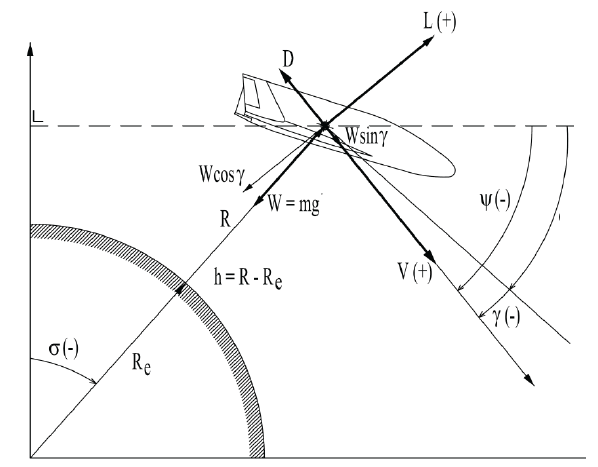
\includegraphics[scale = 1]{Sketch.PNG}

\subsection*{b.}
General equations of motion:
\begin{equation}
    \begin{split}
        m \frac{dV}{dt} = -D - mg\sin{(\gamma)} \\
        m V \frac{d \gamma}{dt} = L - mg \cos{(\gamma)}(1-\frac{V^2}{V_c^2}) \\
        \frac{dr}{dt} = \frac{dh}{dt} = V\sin{\gamma}
    \end{split}
\end{equation}

\subsection*{c.}
For gliding entry, we have that $\gamma \approx 0$ and $\frac{d\gamma}{dt} \approx 0$. If we use this approximations, we get the following form the above equations:


\begin{equation}
    \begin{split}
        m \frac{dV}{dt} = -D \\
        0= L - mg (1-\frac{V^2}{V_e^2}) \\
        \frac{dr}{dt} = \frac{dh}{dt} = 0
    \end{split}
\end{equation}


Now also:

\begin{equation}
    \frac{dV}{dt} = \frac{dV}{ds}\frac{ds}{dt} = V \frac{dV}{ds} = \frac{-D}{m} = \frac{-D}{L} g \frac{L}{mg}
\end{equation}

This then yields:

\begin{equation}
    \frac{dV}{ds} = \frac{- \frac{D}{L}g (1-\frac{V^2}{V_c^2})}{V}
\end{equation}

This gives then:
\begin{equation}
    V dV = - \frac{D}{L}g (1-\frac{V^2}{V_c^2})ds
\end{equation}

For integration, the variable $x = \frac{V^2}{V_c^2}$ can be used, with $dx =\frac{2V}{V_c^2}dV$ giving $dV = \frac{V_c^2}{2V} dx$ and then 

\begin{equation}
    \frac{V_c^2}{2} dx = - \frac{D}{L}g (1-x)ds
\end{equation}

Which can then be written as:

\begin{equation}
     -\frac{L}{D} \frac{1}{g}  \frac{V_c^2}{2} \frac{1}{1-x} dx = ds
\end{equation}

Integration gives:

\begin{equation}
\begin{split}
     \int_{0}^{R_f} ds = \int_{x_1}^{x_2} (-\frac{L}{D} \frac{1}{g}  \frac{V_c^2}{2} \frac{1}{1-x} dx \\
     R_f =  -\frac{L}{D} \frac{1}{g}  \frac{V_c^2}{2} [-\ln{(1-x)}]_{x_1}^{x_2} \\
     R_f =  \frac{L}{D} \frac{1}{g}  \frac{V_c^2}{2} \ln{\frac{(1-x_2)}{1-x_1}} \\
\end{split}     
\end{equation}

Now $x_1 = \frac{V_E^2}{V_c^2}$ and $x_2 = \frac{V_F^2}{V_c^2}$, so:

\begin{equation}
    R_f =  \frac{L}{D} \frac{1}{g}  \frac{V_c^2}{2} \ln{\frac{(1-\frac{V_F^2}{V_c^2})}{1-\frac{V_E^2}{V_c^2}}} \\
\end{equation}

Now $V_F \approx 0$ and $V_c^2 \approx g\cdot R_e$, so ultimately:

\begin{equation}
    \frac{R}{R_e} =  -\frac{1}{2}\frac{L}{D} \ln{1-\frac{V_E^2}{V_c^2})} \\
\end{equation}


\subsection*{d.}
Minimum range to cover: 6000 km. This means that 
\begin{equation}
\begin{split}
      \frac{L}{D} = -2 \cdot \frac{R}{R_e} \frac{1}{ \ln{1-\frac{V_E^2}{V_c^2})}} = -2 \cdot 0.9408 \frac{1}{ \ln{1-\frac{V_E^2}{V_c^2})}} \\    
\end{split}
\end{equation}
Now since $V_E = 0.8 V_c$, we have:
\begin{equation}
   \frac{L}{D} = -1.881 \frac{1}{ \ln{1-0.64}}  = 1.922
\end{equation}

A minimum lift-to-drag ratio of 1.922 is required for the entirety of this flight.

\subsection*{e.}
When the entry velocity $V_E$ approaches the circular velocity $V_c$, the flight range approaches infinity, which is the actual flight range if $V_E = v_c$. This is of little surprise, since this means that the vehicle is actually in orbit and will never land. This limiting case with a non-physical result is thus actually based on physical results.